\section{Evaluation: QDPT on formaldehyde}

\begin{center}
\textit{This section is based on the article at Ref. \citen{ijqc-2005}} \\
\end{center}
{\ }\\
\vspace{-5mm}

A Quasi-Degenerate NEVPT2 evaluation has been conducted over the
formaldehyde molecule. Four electronic states of A$_1$ symmetry have been
considered in the analysis, namely the ground state (1A$_1$), the $n_y \rightarrow
3p_y$ Rydberg state (2A$_1$), the $n_y \rightarrow 3d_{yz}$ Rydberg state
(3A$_1$) and the $\pi \rightarrow \pi^{*}$ valence state (4A$_1$). 

The energy curves for these states have been studied as a function of the CO
distance. The rationale behind this study is to analyze the qualitative
behavior of the avoided crossing of the potential energy curves arising from
these states.  A simple CASSCF wavefunction does not keep fully into account
the dynamic correlation needed for the description of the ground and $\pi
\rightarrow \pi^{*}$ state. These states require higher correlative
corrections than the ones needed by the Rydberg states, due to the high
average distance of the promoted electron from the molecular framework in
the Rydberg case.  Also, the large mixing occurring between Rydberg and
valence states invokes the need for a Quasi-Degenerate treatment.

A state averaged CASSCF procedure with an active space of six electrons in
seven orbitals has been performed. The interested active orbitals are the
$\sigma$, $\sigma^{*}$, the $\pi$, $\pi^{*}$, the $n_y$ and the $3p_y$ and
$3d_{yz}$ Rydberg orbitals. To describe the potential curve, CO bond
distances from 2.00 bohr to 3.40 bohr have been considered, with a step of
0.1 bohr.  Occasionally, the step length has been reduced to address
particular features of the curves. Other geometrical parameters have been
kept fixed at the values obtained by a HF/MP2 complete optimization with
the same basis set.

The basis set is the ANO-1, augmented with a Rydberg set of functions built
as detailed in Sec. \ref{sec:rydberg_procedure}. The contraction scheme
produced a set [$1s1p1d$] from a decontracted set of diffuse functions
[$8s8p8d$], centered on the charge centroid evaluated at the ground state
geometry. The position of the centroid is unchanged during the CO
elongation, given its marginal influence on the final results.

The procedure is briefly presented here: for each molecular geometry an
averaged CASSCF evaluation has been performed, producing a set of averaged
molecular orbitals. For each state, the average orbitals are brought in
canonical form in the inactive set. 

\begin{center}
\begin{figure}[ht]
\begin{center}
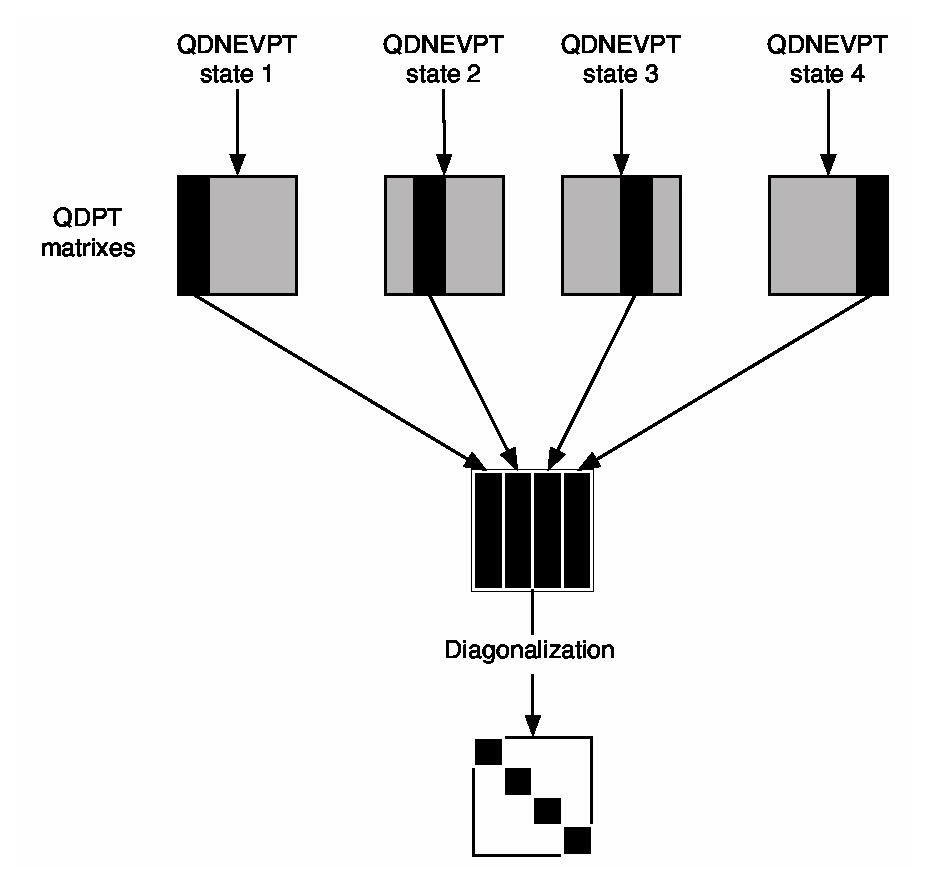
\includegraphics[width=10cm]{03_nevpt/images/qdpt_diagram-gimped.eps}
\end{center}
\caption{\footnotesize The computational scheme for the evaluation of the
Quasi Degenerate treatment. Four different QDPT matrixes are obtained by the
procedure, each one referring to a particular state. A single column is
extracted from each matrix and gathered in a final matrix which is
diagonalized. }
\label{fig:qdpt_diagram}
\end{figure}
\end{center}


This procedure provides four orbital sets, which are used in the Quasi-Degenerate evaluation. Four matrixes are obtained (refer to Fig.
\ref{fig:qdpt_diagram}) each one referring to a particular state. To build
the final effective Hamiltonian matrix to be diagonalized, the following
steps must be applied:
\begin{enumerate}
\item decompose the four matrixes columnwise
\item extract the column number $n$ from the matrix referring to the $n$-th
electronic state
%\item check if coupling (non-diagonal) elements have the correct sign
\item build a final matrix, made of the obtained columns
\item diagonalize it to obtain the final energies and coefficients
\end{enumerate}

%Some explanation have to be reported for the third point: non-diagonal
%elements refer to integrals
%$\braket{\Psi_n^{(0)}}{\ham_{\mbox{eff}}}{\Psi_m^{(0)}}$. The computational
%procedure followed by each matrix is the same, but the final wavefunctions
%can differ in sign. As an example, in the evaluation of the first state the
%element $\braket{\Psi_2^{(0)}}{\ham_{\mbox{eff}}}{\Psi_1^{(0)}}$ can be
%referred to wavefunction with the same sign. For the evaluation of
%$\braket{\Psi_1^{(0)}}{\ham_{\mbox{eff}}}{\Psi_2^{(0)}}$, the sign of
%$\Psi_2^{(0)}$ can be different. A direct comparison of the two integrals is
%not possible, due to their different absolute values.

%A possible solution is to choose as a reference the evaluation matrix provided
%by the first electronic state.  Orbitals for the remaining states are
%preserved only in the inactive part, while the active part is replaced with
%the orbitals from the first set. This approach is formally correct since the
%CAS evaluation is a Full-CI inside this orbital space, and the NEVPT
%treatment is invariant for orbital mixing inside the active block. A quick
%check for the sign of the CI coefficients now can be performed, an
%appropriate sign adaptation for each element of the final matrix. The
%procedure has been implemented as an automatic bash script to prevent
%errors from a manual process.

The curves obtained at CASSCF level are represented in Fig.
\ref{fig:formaldehyde_cas_curve}. The main feature is the behavior of the
$\pi \rightarrow \pi^{*}$ 4A$_1$ state with respect to 2A$_1$ and 3A$_1$
Rydberg states. The Rydberg states are nearly parallel to the ground state.
This is expected since the electron is promoted from a non-bonding orbital
to a distant one, introducing very little destabilization in the electronic
asset that governs the molecular geometry.

On the other hand, the valence
excited state introduces a serious variation in this asset, moving from a
double bond situation to a nearly single bond situation. This imposes a
steep elongation of the bond, and the potential energy curve for this state
crosses the Rydberg ones. Due to interaction between these states, an
avoided crossing situation occurs, producing the resulting diagram.
\vspace{-3mm}
\begin{center}
\begin{figure}[ht]
\begin{center}
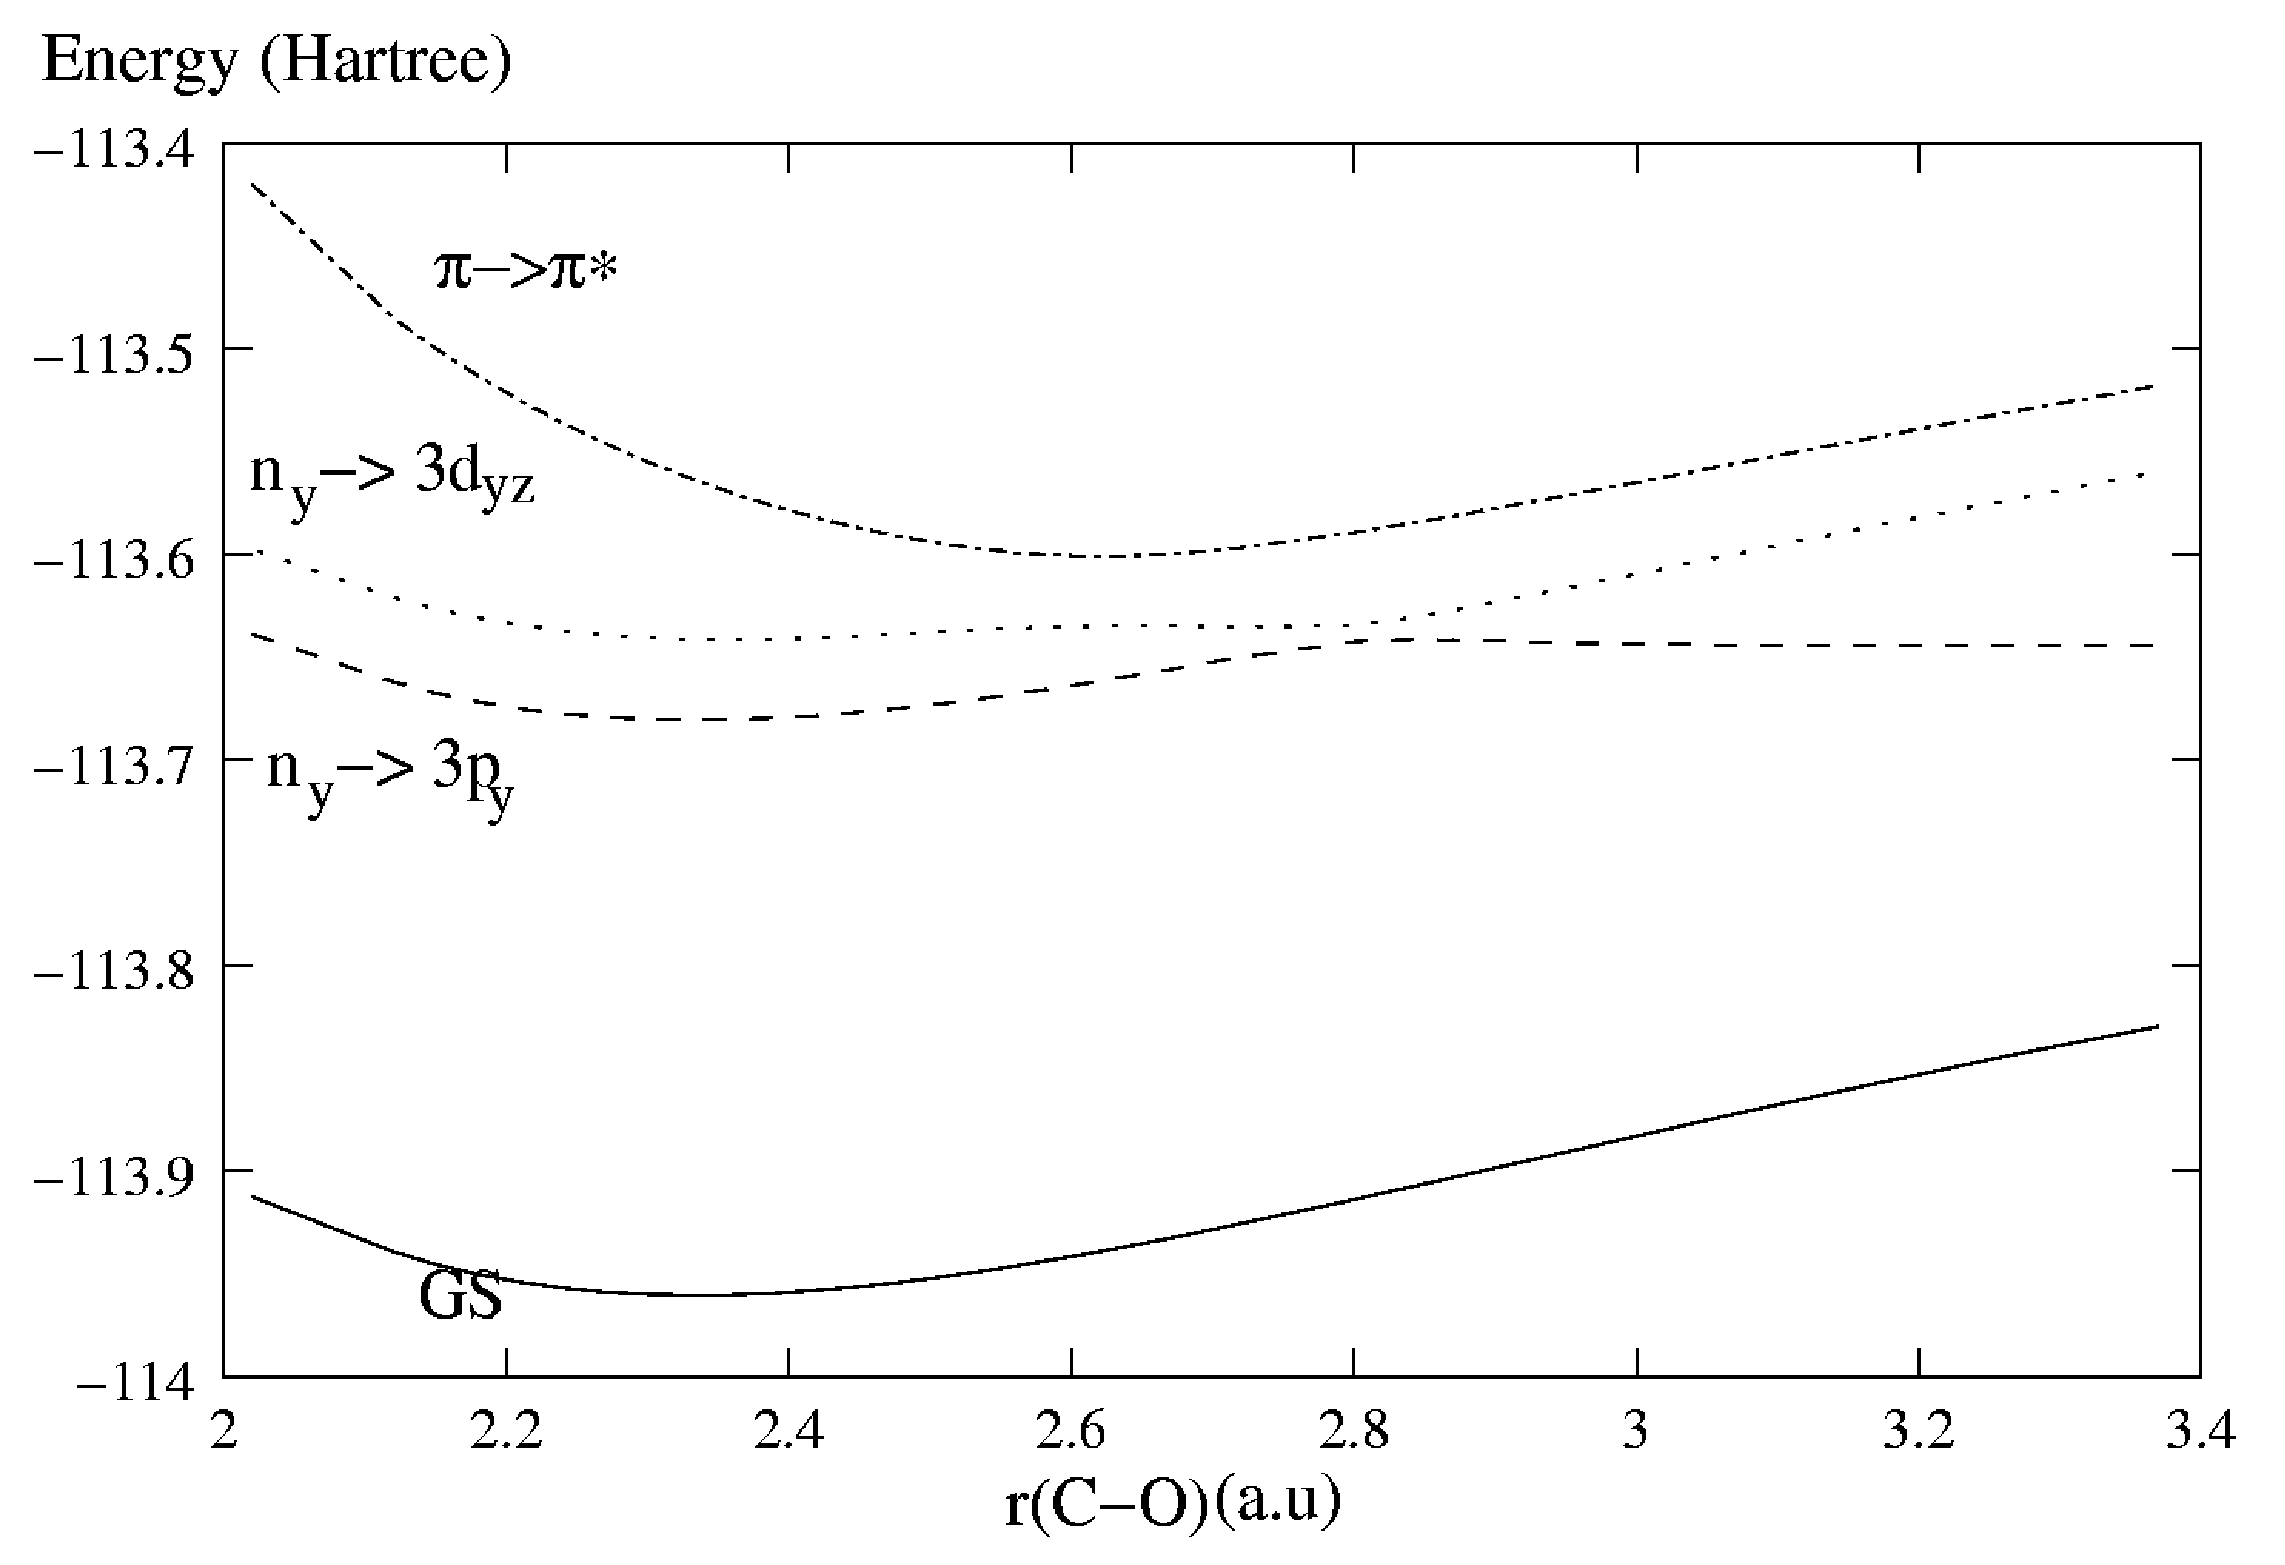
\includegraphics[width=11cm,keepaspectratio]{03_nevpt/images/formaldehyde-cas-curve.eps}
\end{center}
\caption{\footnotesize CASSCF energy curves for the ground state, $n \rightarrow$
Rydberg and $\pi \rightarrow \pi^{*}$ of formaldehyde with respect to the CO
bond lenght.}
\label{fig:formaldehyde_cas_curve}
\end{figure}
\end{center}

Applying the perturbation treatment, it is expected that the correlation for
valence states will be higher than for Rydberg states. 
As a direct consequence the avoided crossings move at shorter distances, see
Fig.~\ref{fig:formaldehyde_qdpt_curve}, solid line. The same plot also
reports the results produced by a Single-State NEVPT2 treatment (dotted
lines). These curves have no physical meaning and behave in incorrect ways.
The presence of non-diagonal elements in the effective Hamiltonian matrix
fixes the invalid behavior, allowing the wavefunction to interact at NEVPT2
level.
\vspace{-3mm}
\begin{center}
\begin{figure}[ht]
\begin{center}
\includegraphics[width=11cm]{03_nevpt/images/formaldehyde-qdpt-curve.eps}
\end{center}
\caption{\footnotesize Energy curves for the ground state, $n \rightarrow$
Ryd and $\pi \rightarrow \pi^{*}$ of formaldehyde with respect to the CO
bond lenght. The solid line represents the QD-NEVPT evaluation. The dotted
lines report the Single-State evaluation.}
\label{fig:formaldehyde_qdpt_curve}
\end{figure}
\end{center}

\vspace{-3mm}
A final consideration must however be raised working with a more accurate
point grid. The plot in Fig. \ref{fig:qdpt_error} represents the 2A$_1$ and
3A$_1$ Rydberg states at QD-NEVPT level of theory, using a finer grid (step
0.01 bohr) between 2.7 bohr and 2.9 bohr. An incorrect behavior is observed
for both curves. This behavior is not appreciable in the Ground
State and $\pi \rightarrow \pi^{*}$ curves. For comparison, the avoided
crossing at CASSCF level is reported between the QDPT curves. The CASSCF
curves have been transposed in energy to fit correctly into the plot.

It can be noted that the position of the incorrect behavior matches the
position of the avoided crossings at CASSCF level. This is probably due to a
wrong estimation of the coupling between the curves. Tests performed with
larger CAS spaces lead to a reduction of the incorrect behavior, which
expresses itself at shorter distances, following again the avoided crossing.
A possible explanation of the problem lies in a bad description of the
zero-order situation, and the inability for the NEVPT2 treatment to fully
recover the coupling. This brings a ``memory-effect'' on the QDPT curves.  A
non trivial solution to the problem could be looked for in the definition of an
iterative procedure, where the QD-NEVPT treatment is performed on the
refined wavefunctions obtained from the previous step. 
\vspace{-3mm}
\begin{center}
\begin{figure}[ht]
\begin{center}
\includegraphics[width=7cm,keepaspectratio,angle=270]{03_nevpt/images/qdpt_error.eps}
\end{center}
\caption{\footnotesize The incorrect behavior of the 2A$_1$ (cross symbol)
and 3A$_1$ (star symbol) Rydberg states at QD-NEVPT level, with respect to
the elongation of the CO bond. A grid step of 0.01 bohr between 2.7 and 2.9
bohr has been used.
Between the curves the plot also depicts the CASSCF avoided crossing taking
place at the same bond length. The avoided crossing curves have been
transposed to better fit into the plot. } \label{fig:qdpt_error}
\end{figure}
\end{center}

\vspace{-6mm}

